\documentclass[sigconf]{acmart}

\usepackage{hyperref}

%\usepackage{endfloat}
%\renewcommand{\efloatseparator}{\mbox{}} % no new page between figures

\usepackage{booktabs} % For formal tables

\settopmatter{printacmref=false} % Removes citation information below abstract
\renewcommand\footnotetextcopyrightpermission[1]{} % removes footnote with conference information in first column
\pagestyle{plain} % removes running headers

\graphicspath{ {./images/}}
\usepackage{subcaption}
\usepackage[table]{xcolor}
\usepackage{url}

\begin{document}
\title{Analyzing everyday challenges of people with visual impairments}


\author{Tousif Ahmed}
\orcid{HID237}
\affiliation{%
\institution{Indiana University}
  \streetaddress{150 S Woodlawn Avenue}
  \city{Bloomington} 
  \state{Indiana} 
  \postcode{47405}
}
\email{touahmed@indiana.edu}



\begin{abstract}
       People with visual impairments face varieties of problem in their daily lives. Nowadays, modern technology especially camera-based technologies are helping people with visual impairment in their everyday tasks ranging from daily household activity to navigation. Users are using camera based applications where they are sharing photos and asking questions. Based on the asked question and shared photo, automated tools or human crowd workers are helping the visually impaired people in their tasks. By exploring the questions, it is possible to understand the problems and challenges of people with visual impairments. However, the volume of such data makes it impossible to analyze the questions manually.  Big data analytics could help us to understand the challenges of people with visual impairments. To understand the challenges, we analyzed the VizWiz data set which contains more than 33,500 questions asked by people with visual impairments. In this paper, we report on the data and shed light on the challenges.  

\end{abstract}

\keywords{E534, HID 237,  Big Data, Accessibility Issues, People with Visual Impairments}


\maketitle


\section{Introduction}
People with visual impairments face a variety of problems in their daily lives and need assistance. They need assistance with detecting objects, identifying money, navigation, transportation, household activities, cooking, and various other activities. Sighted person on rely on vision on so many things that it is almost impossible to visualize and understand the problems of people with visual impairments. Although there are variety of tools available to simulate the challenges and experiences of people with visual impairments, the challenges of people with visual impairments is not well understood. To help visually impaired people with technologies, we need to understand their problem first.

One possible to understand the challenges of people with visual impairments is qualitative analysis or ethnographic studies with people with visual impairments. Simply, researchers can follow or conduct interviews with people with visual impairments. Although qualitative studies are widely accepted research methods, it has limitations. Specially to understand the problems of people with visual impairments, qualitative studies have severe limitations. As the challenges vary with the experiences of people with visual impairments, these studies can not capture or depict the whole picture. Besides, these studies are very expensive and need ample human effort. Therefore, we need a better way to understand the challenges of people with visual impairments.

Big data analytics could be a potential alternative. To understand how big data can help people with visual impairments, we need to understand the backgroungd first. Nowadays, people with visual impairments uses different technologies for their problems.A wide range of technologies such as talking watch\footnote{https://www.maxiaids.com/talking-watches}, braille reader\footnote{\url{http://www.afb.org/prodBrowseCatResults.aspx?CatID=43}}, navigation helper \footnote{\url{http://www.gdp-research.com.au/}} are available in the market to help the visually impaired in their daily tasks. Since the introduction of smartphone, smartphone based applications gained huge popularities among people with visual impairments. Now, mobile and smartphone applications like Seeing AI~\cite{seeingai}, AiPoly~\cite{aipoly},LookTel~\cite{looktel}, and other such camera based applications are helping people with visual impairmentsin object recognition, face recognition, color detection, human emotion detection, activity recognition, and other such tasks that was not possible before. Figure ~\ref{fig:seeingai} depicts an example from Seeing AI which shows that how camera based applications are helping people with visual impairments by describing nearby person's activitty (Figure ~\ref{fig:ios}) and their facial emotions (Figure ~\ref{fig:facial}) .
\begin{figure}[tbp]
        \centering
        \begin{subfigure}[b]{0.4\columnwidth}
                %\includegraphics[width=\textwidth]{figures/appPermissions.pdf}  
                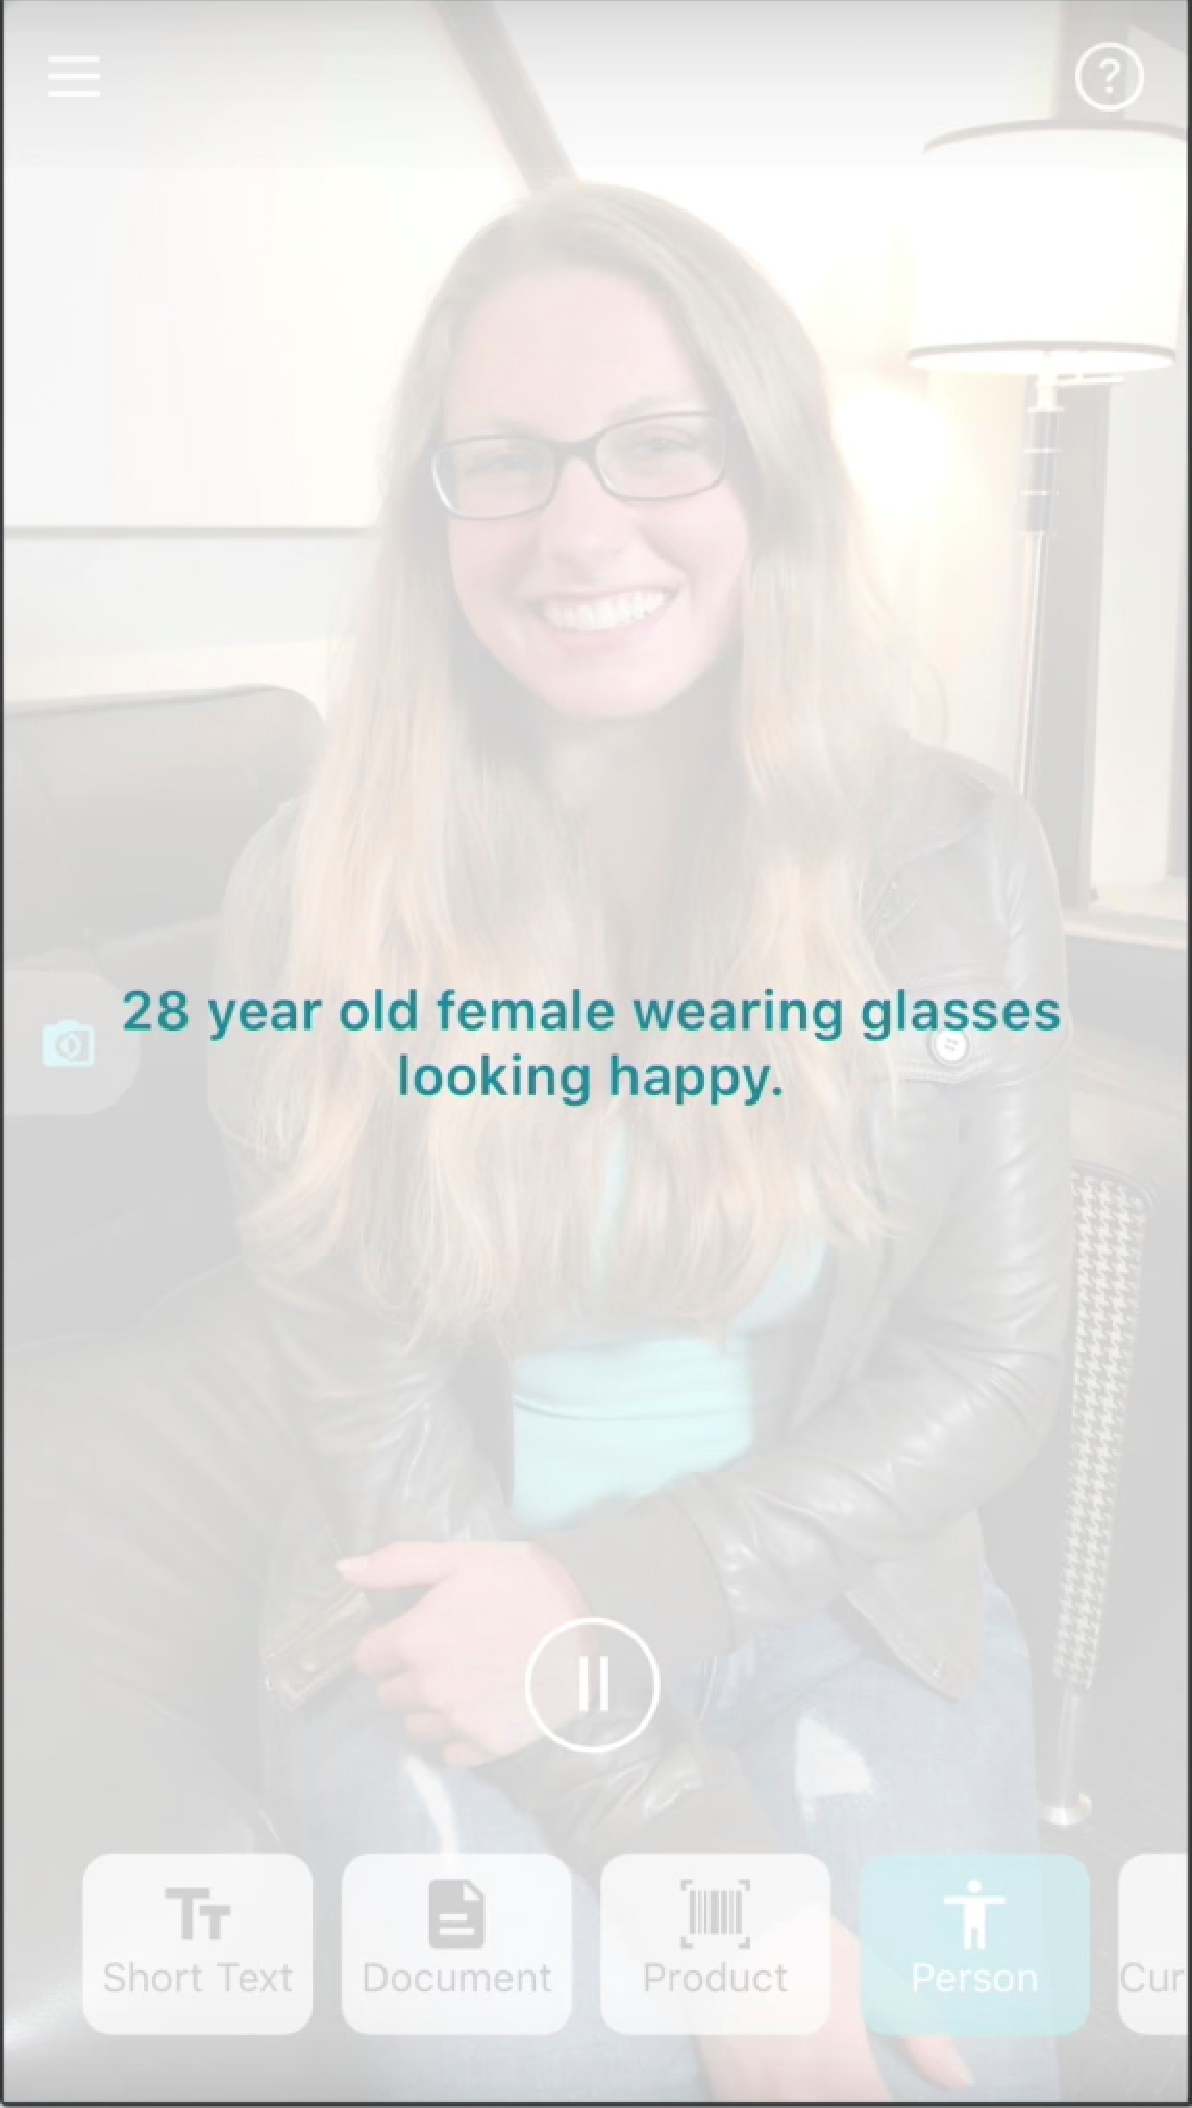
\includegraphics[width=\textwidth]{project/images/facial.pdf}  
                \caption{Age, gender, appearance, and facial expression} 
                  \label{fig:facial}   
        \end{subfigure}%
        ~ 
        \begin{subfigure}[b]{0.4\columnwidth}
                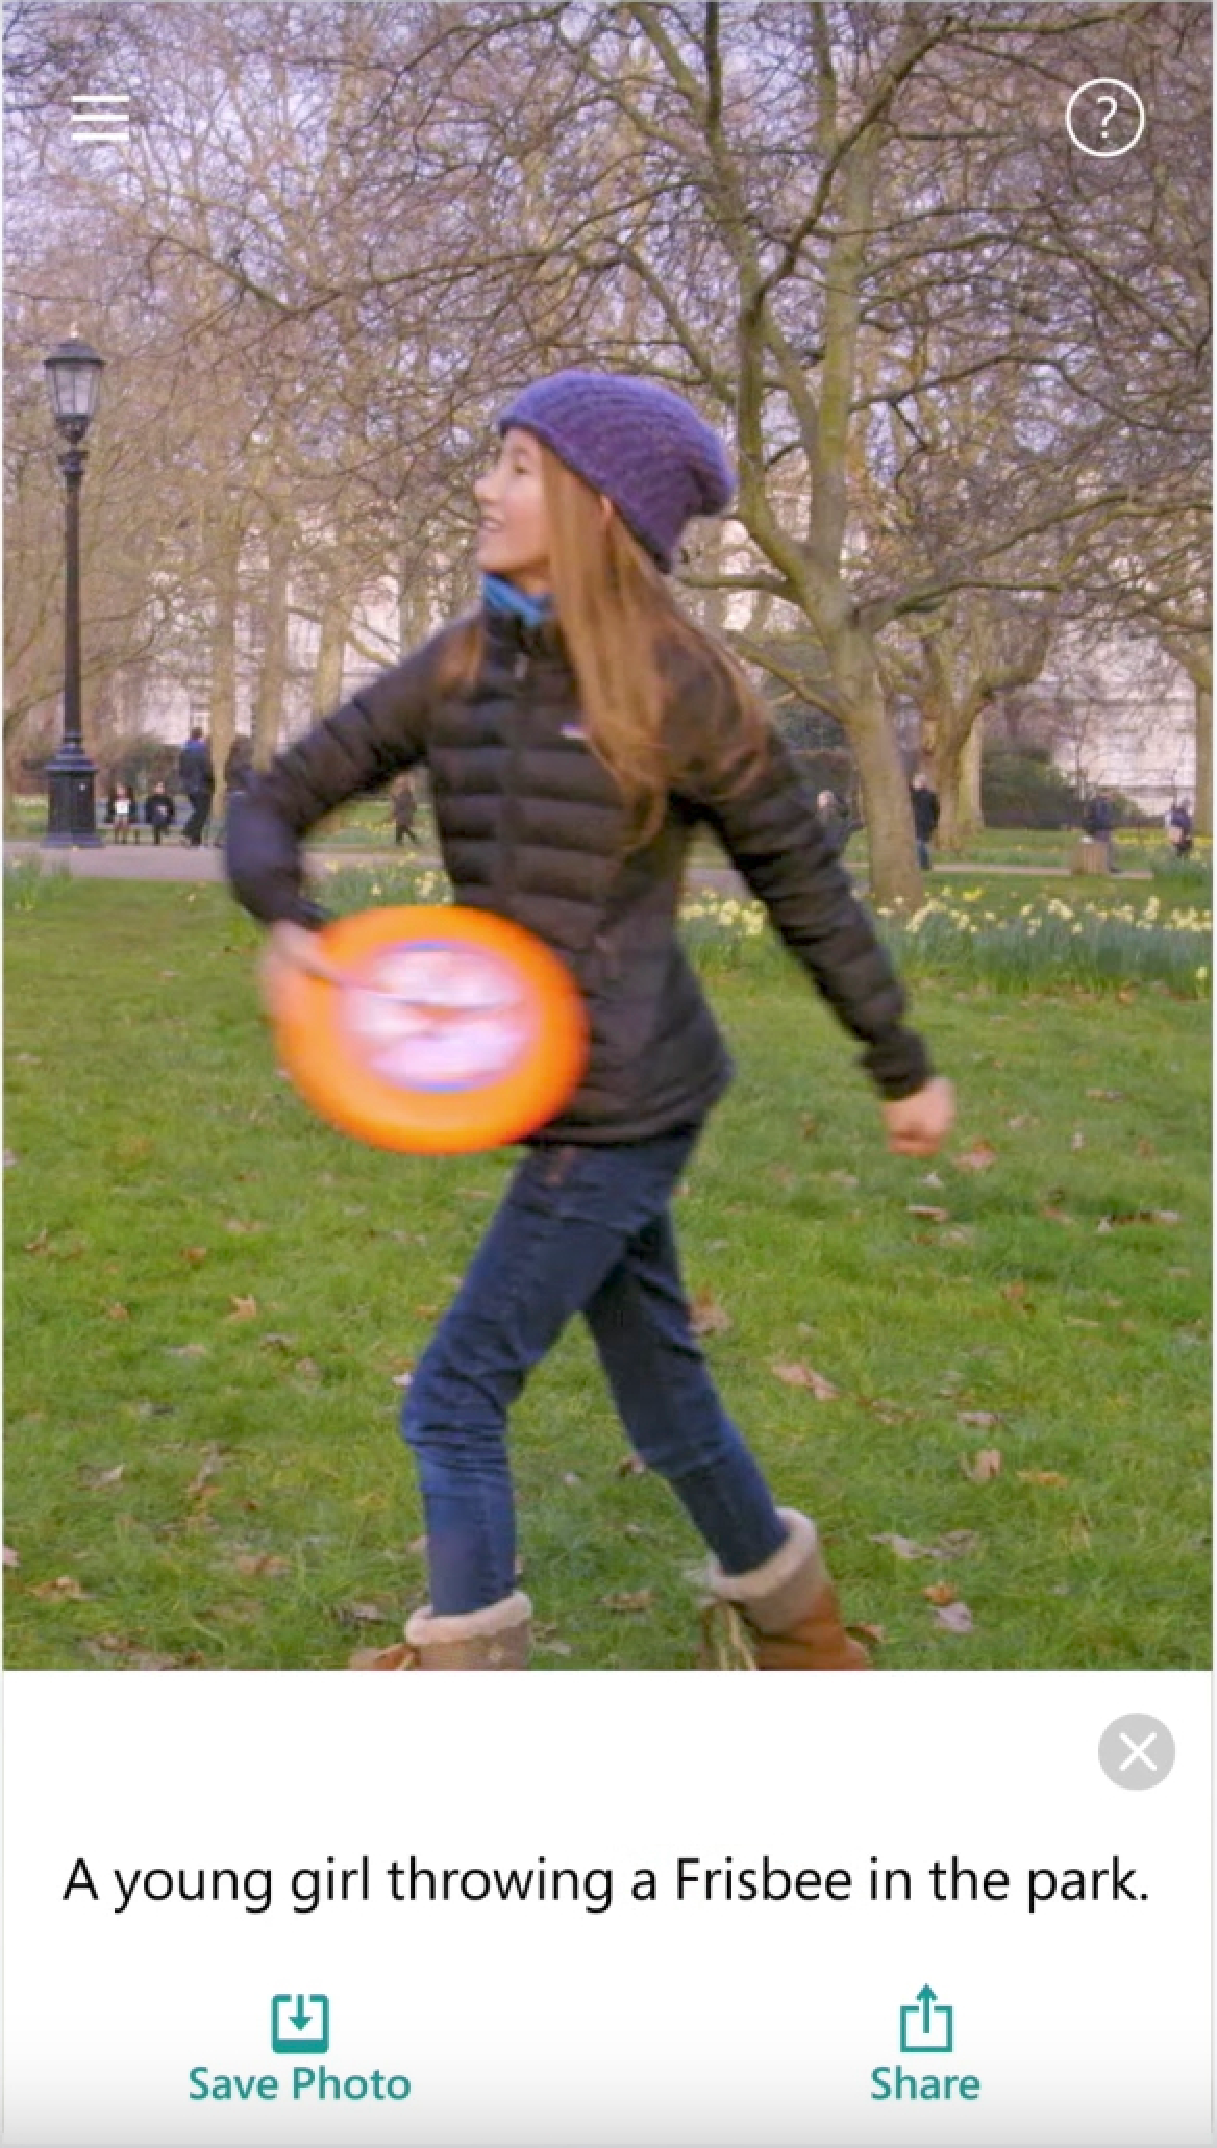
\includegraphics[width=\textwidth]{project/images/activity2.pdf}  
                 \caption{Age, gender, and activity of a nearby person}
                  \label{fig:ios}      
        \end{subfigure}%
        \caption{Seeing AI providing various information about people nearby~\cite{seeingai}.} 
        %Android currently displays the requested permissions during the app installation process. iOS  allows selective disabling of permissions for installed apps.}
        \label{fig:seeingai}
\end{figure}

Most of the camera assisted assitive applications works in one simple way.The user uploads an intended photo and asks a question about that. Applications have it's simple iq engine which tries to answer the problem first. If it's not able to answer that question, it shares the questions and images with the user's friends and family. Sometimes, the image is shared with a web based human worker. This crowd wroker is essential for such system, because the iq engine is not sophisticated yet. We can not completely trust the automated approaches.  Besides, visually impaired user's can not efficiently take photos. Sometimes they point at totally wrong objetcts or items, sometimes they share blurry photos, and even sometimes the question does not match with the photos~\cite{Jayant:2011,Bigham:2010,Harada:2013}. Therefore, to give a correct answer of the questions, technologies require human intelligence. Questions and answer based applications like TapTapSee~\cite{taptapsee} and VizWiz~\cite{Bigham:2010} uses this approach. LookTell~\cite{looktel} and BeMyEyes does not have any automated approach, it directly broadcasts the video feed to the volunteers and volunteers answer their questions. Some applications are trying to move towards the fully automated approach, however, due to the limitations of automated approaches they did not gain much popularity yet. 

Human based systems have privacy issues, because these users are uploading their photos which may contain sensitive information. Often they ask about medical information, their address, and various other sensitive information which can be exploited by the malicious crowd workers. Even sometimes, the users shares their credit card image and asks the system to about their credit card information which have severe privacy and security implications. Moreover, cameras and images shared by them can be extremely risky for people with visual impairments, becuase often they do not know the contents of the photo. Photos can be uploaded in error, sensitive data can be shared unintentionally. Ahmed et al.~\cite{Ahmed:2016} reported a scary story of one of the VizWiz users, who accidentally shared her naked photo with a crowd worker. Such evidents suggestsb that such systems has severe privacy and security implications. However, visually impaired needs such tool in their daily lives. Therefore, the ideal solution would be an completely automated approach. However, to design a flawless system we need to improve the existing tools first and we need to understand the challenges first.

The challenges of people with visual impairments can be easily understood from the images uploaded and questions asked by the user. Although it is extremely difficult for people with visual impairments to take a good photo, still they are using these tools because of their challenges. Therefore, the data uploaded in these applications are probably a good way to understand the challenges. However, due to the volume of the data it is not possible to manually identify the problems. Therefore, big data analytics can be helpful in this context to understand the challenges of people with visual impairments. However, due to privacy issues all but one data sets are not publicly available. 

In this paper, we analyzed the VizWiz data set containing more than 35000 images and questions~\cite{Bigham:2010}. Based on the questions asked, we tried to categorize their problems which eventually help the researchers to design and develop a fully automated system.Previous researches~\cite{Brady:2013} explored the same problem with the same data set. However, they only explored 1000 images and performed a qualitative study and idetified four categories of problem. Since manula analyis is not possible on 35000 data, we used big data tools to automatically analyze the questions and images. In this paper, we report on analysis performed and the visual challenges of people with visual impairments


\begin{acks}

The authors would like to thank Professor Gregor von Laszewski for helping us with the instruction and resources that were required to complete this paper. We would also to like to thank the associate instructors for being available on the course website all the time and helping us with their answers.

\end{acks}



\bibliographystyle{ACM-Reference-Format}
\bibliography{report} 
\newpage
\appendix

%We include an appendix with common issues that we see when students submit papers. One particular important issue is not to use the underscore in bibtex labels. Sharelatex allows this, but the proceedings script we have does not allow this.

%When you submit the paper you need to address each of the items in the
%issues.tex file and verify that you have done them. Please do this
%only at the end once you have finished writing the paper. To d this
%cange TODO with DONE. However if you check something on with DONE, but
%we find you actually have not executed it correcty, you will receive
%point deductions. Thus it is important to do this correctly and not
%just 5 minutes before the deadline. It is better to do a late
%submission than doing the check in haste. 

\section{Issues}

\DONE{Example of done item: Once you fix an item, change TODO to DONE}

\subsection{Assignment Submission Issues}

    \TODO{Do not make changes to your paper during grading, when your repository should be frozen.}

\subsection{Uncaught Bibliography Errors}

    \DONE{Missing bibliography file generated by JabRef}
    \DONE{Bibtex labels cannot have any spaces, \_ or \& in it}
    \DONE{Citations in text showing as [?]: this means either your report.bib is not up-to-date or there is a spelling error in the label of the item you want to cite, either in report.bib or in report.tex}

\subsection{Formatting}

    \TODO{Incorrect number of keywords or HID and i523 not included in the keywords}
    \TODO{Other formatting issues}

\subsection{Writing Errors}

    \DONE{Errors in title, e.g. capitalization}
    \DONE{Spelling errors}
    \TODO{Are you using {\em a} and {\em the} properly?}
    \DONE{Do not use phrases such as {\em shown in the Figure below}. Instead, use {\em as shown in Figure 3}, when referring to the 3rd figure}
    \DONE{Do not use the word {\em I} instead use {\em we} even if you are the sole author}
    \TODO{Do not use the phrase {\em In this paper/report we show} instead use {\em We show}. It is not important if this is a paper or a report and does not need to be mentioned}
    \DONE{If you want to say {\em and} do not use {\em \&} but use the word {\em and}}
    \DONE{Use a space after . , : }
    \DONE{When using a section command, the section title is not written in all-caps as format does this for you}\begin{verbatim}\section{Introduction} and NOT \section{INTRODUCTION} \end{verbatim}

\subsection{Citation Issues and Plagiarism}

    \DONE{It is your responsibility to make sure no plagiarism occurs. The instructions and resources were given in the class}
    \DONE{Claims made without citations provided}
    \DONE{Need to paraphrase long quotations (whole sentences or longer)}
    \DONE{Need to quote directly cited material}

\subsection{Character Errors}

    \DONE{Erroneous use of quotation marks, i.e. use ``quotes'' , instead of " "}
    \DONE{To emphasize a word, use {\em emphasize} and not ``quote''}
    \DONE{When using the characters \& \# \% \_  put a backslash before them so that they show up correctly}
    \DONE{Pasting and copying from the Web often results in non-ASCII characters to be used in your text, please remove them and replace accordingly. This is the case for quotes, dashes and all the other special characters.}
    \DONE{If you see a figure and not a figure in text you copied from a text that has the fi combined as a single character}

\subsection{Structural Issues}

    \DONE{Acknowledgement section missing}
    \DONE{Incorrect README file}
    \DONE{In case of a class and if you do a multi-author paper, you need to add an appendix describing who did what in the paper}
    \TODO{The paper has less than 2 pages of text, i.e. excluding images, tables and figures}
    \TODO{The paper has more than 6 pages of text, i.e. excluding images, tables and figures}
    \TODO{Do not artificially inflate your paper if you are below the page limit}

\subsection{Details about the Figures and Tables}

    \DONE{Capitalization errors in referring to captions, e.g. Figure 1, Table 2}
    \DONE{Do use {\em label} and {\em ref} to automatically create figure numbers}
    \DONE{Wrong placement of figure caption. They should be on the bottom of the figure}
    \DONE{Wrong placement of table caption. They should be on the top of the table}
    \DONE{Images submitted incorrectly. They should be in native format, e.g. .graffle, .pptx, .png, .jpg}
    \DONE{Do not submit eps images. Instead, convert them to PDF}

    \DONE{The image files must be in a single directory named "images"}
    \DONE{In case there is a powerpoint in the submission, the image must be exported as PDF}
    \DONE{Make the figures large enough so we can read the details. If needed make the figure over two columns}
    \DONE{Do not worry about the figure placement if they are at a different location than you think. Figures are allowed to float. For this class, you should place all figures at the end of the report.}
    \DONE{In case you copied a figure from another paper you need to ask for copyright permission. In case of a class paper, you must include a reference to the original in the caption}
    \DONE{Remove any figure that is not referred to explicitly in the text (As shown in Figure ..)}
    \DONE{Do not use textwidth as a parameter for includegraphics}
    \DONE{Figures should be reasonably sized and often you just need to
  add columnwidth} e.g. \begin{verbatim}/includegraphics[width=\columnwidth]{images/myimage.pdf}\end{verbatim}



\end{document}
